\documentclass[]{scrartcl}
\usepackage{Preamble}

\setcounter{section}{4}
\newcommand{\exercise}{Exercise \thesection}
\newcommand{\duedate}{2020-12-14, 23:59}

\begin{document}
\section*{\exercise}

To compile: unzip our uploaded code, and run \verb|make| inside \verb|code/|.
The slurm scripts are stored inside \verb|code/slurm/|.
To debug: run the debug outputs (\verb|*.dbg|) and attach gdb to respective pids

\subsection{Reading}
\subsection{Matrix multiply --- parallel version using MPI}\label{ssec:mmul_parallel}
\subsection{Matrix multiply --- scaling process count}\label{ssec:mmul_proc}

The program of \autoref{ssec:mmul_parallel} was tested on its scalability with an increasing number of processes.
The times and speedups in \autoref{tab:proc} were observed for 2000x2000 matrices with 100 repetitions.

\begin{table}[ht]
    \centering
    \begin{tabular}{rr}
\toprule
 nodes &  GFLOPS64/s \\
\midrule
     1 &     1.55161 \\
     3 &     2.28341 \\
     5 &     2.89719 \\
     7 &     3.89113 \\
     9 &     4.90389 \\
    11 &     5.42166 \\
    13 &     6.30550 \\
    15 &     7.30316 \\
\bottomrule
\end{tabular}

    \caption{Scaling by Processes in numbers}\label{tab:proc}
\end{table}

For this Example a step is visible before 6 pocesses, most likeley because here only one node is used and we are reaching its maximum. Starting with 6 processes, this maximum is increased.

\begin{figure}[H]
    \centering
    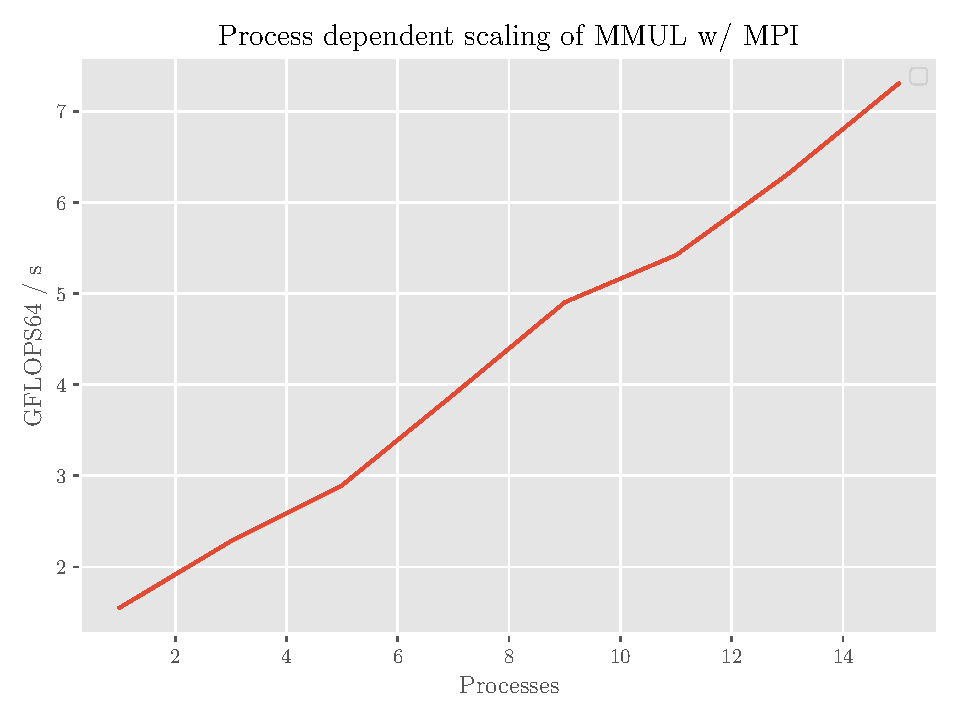
\includegraphics[width=\linewidth]{img/scaling_proc.pdf}
    \caption{Scaling Process Count}%
    \label{fig:scaling_proc}
\end{figure}

\subsection{Matrix multiply --- scaling problem size}
In addition to the process scaling in \autoref{ssec:mmul_proc}, the scaling by problem size was also observed. The observed numbers are shown in \autoref{tab:prob}, here each test was run for both 10 and 16 processes as well as repeated 10 times.

\begin{table}[ht]
    \centering
    \begin{tabular}{llrr}
\toprule
     &    & \multicolumn{2}{l}{GFLOPS64/s} \\
     &    &       mean &    std \\
dim & nodes &            &        \\
\midrule
128  & 10 &      0.778 &  0.058 \\
     & 16 &      0.407 &  0.012 \\
256  & 10 &      3.056 &  0.249 \\
     & 16 &      2.523 &  0.106 \\
512  & 10 &      5.164 &  0.204 \\
     & 16 &      6.505 &  1.947 \\
1024 & 10 &      4.529 &  0.687 \\
     & 16 &      3.231 &  1.393 \\
2048 & 10 &      5.281 &  0.132 \\
     & 16 &      7.451 &  0.967 \\
4096 & 10 &      5.593 &  0.054 \\
     & 16 &      8.601 &  0.128 \\
\bottomrule
\end{tabular}

    \caption{Scaling by Problem Size in numbers}\label{tab:prob}
\end{table}
\begin{figure}[H]
    \centering
    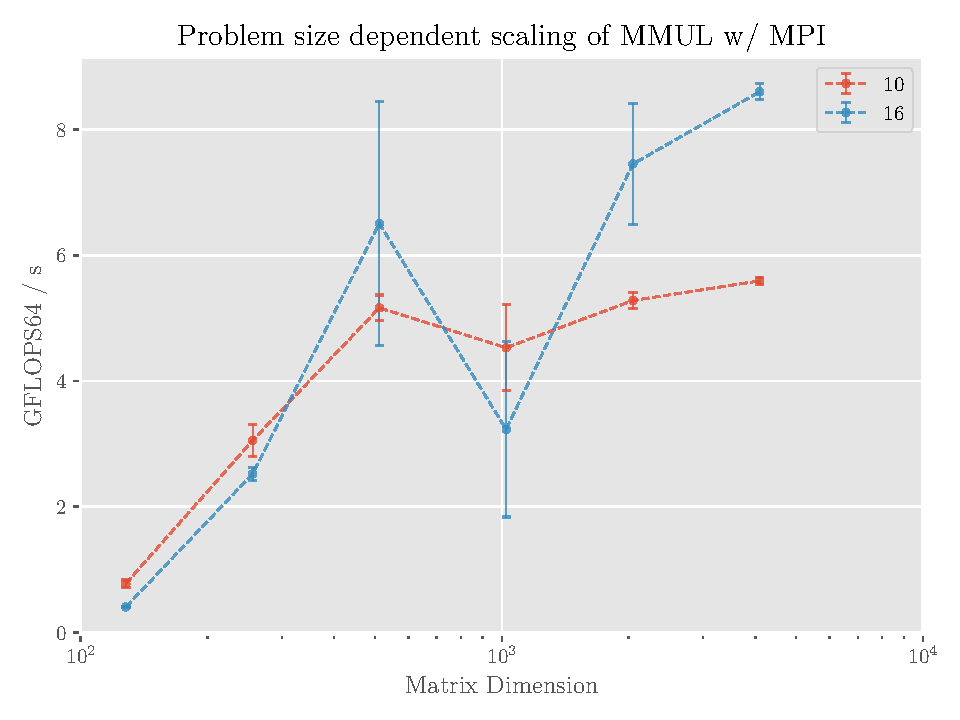
\includegraphics[width=\linewidth]{img/scaling_prob.pdf}
    \caption{Scaling Problem Size}%
    \label{fig:scaling_prob}
\end{figure}

\end{document}
